\documentclass[10pt,fleqn]{article} % Default font size and left-justified equations
\usepackage[%
    pdftitle={Introduction à l'algorithmique et à la programmation},
    pdfauthor={Xavier Pessoles}]{hyperref}

\newcommand{\repRel}{../../../../}
\input{\repRel/Style/packages}
\input{\repRel/Style/new_style}
\input{\repRel/Style/macros_SII}
\input{\repRel/Style/environment}


\newcommand{\macrocomp}{macro_competences}
\newcommand{\comp}{competences}
\newcommand{\td}{fichier_td}
\newcommand{\repExo}{dossier}
\newcommand{\repStyle}{\repRel/Style}

\def\xxYCartouche{-2.25cm}
\def\xxYongletGarde{.5cm}
\def\xxYOnget{.9cm}

\begin{document}

\livrettrue
\graphicspath{{\repStyle/png/}}
\input{\repStyle/Info_01_Entete}
\graphicspath{{\repStyle/png/}{\repRel/Informatique/Semestre_01/01_Bases/Cours/images/}}
%\input{\repRel/Informatique/Semestre_01/01_Bases/Cours/01_Bases.tex}


\def\xxcompetences{}
\def\xxfigures{}
\def\xxchapitre{}
\def\xxtitreexo{Activités pratiques}
\def\xxsourceexo{}
\def\xxactivite{TP 05 \ifprof  -- Corrigé \else \fi}
\input{\repRel/Style/pagegarde_TD}


\proffalse
\vspace{5cm}
\pagestyle{fancy}
\thispagestyle{plain}

\graphicspath{{\repStyle/png/}{\repRel/Informatique/Exercices/S1_07_Images/03_TraitementPNG/}}
\input{\repRel/Informatique/Exercices/S2_05_RepresentationNombres/01_observations.tex}
\exer{Détermination du nombre de bit de la mantisse d'un flottant}

On se propose de vérifier que le stockage de la mantisse d'un flottant \texttt{python} s'effectue sur 52 bits.
On note $m_c=m-1$, \texttt{m} étant la mantisse du flottant. \texttt{mc} est la valeur stockée en mémoire en binaire.
L'idée est de se servir du nombre $0,5$ dont on connait parfaitement la décomposition binaire :

\begin{center}
$0,5=\frac{1}{2}=1 \times \frac{1}{2} + 0 \times \frac{1}{4} + 0 \times \frac{1}{8}... $
\end{center}

On observe qu'en divisant $m_c$ successivement par 2 on obtient :
\begin{center}
$
\begin{array}{l l l l}
m_c=0.5 & m=1.5 & \mbox{stockée en mémoire sous la forme} & 1000...000\\
m_c=0.25 & m=1.25 & \mbox{stockée en mémoire sous la forme} & 0100...000\\
m_c=0.125 & m=1.125 & \mbox{stockée en mémoire sous la forme} & 0010...000\\
...\\
m_c=0.00...1 & m=1.00...1 & \mbox{stockée en mémoire sous la forme} & 0000...001\\
\end{array}
$
\end{center}

Au bout d'un nombre suffisamment grand de divisions par 2 le chiffre 1 disparait complètement. En comptant le nombre de divisions par 2 nécessaires pour aboutir à 0, on a accès au nombre de bits disponibles pour coder $m_c$.\\
On propose l'algorithme suivant :

\begin{tabular}{p{1cm}|p{1cm}|p{5cm}}
& \multicolumn{2}{l}{Initialisation (à compléter)} \\
& \multicolumn{2}{l}{\textbf{Tant que} $1+m_c \neq 1$ \textbf{faire}} \\
&& $m_c \leftarrow m_c/2 $\\
&& $i \leftarrow i+1 $\\
& \multicolumn{2}{l}{\textbf{fin}} \\
& \multicolumn{2}{l}{\textbf{retourner } $i$} \\
\end{tabular}


%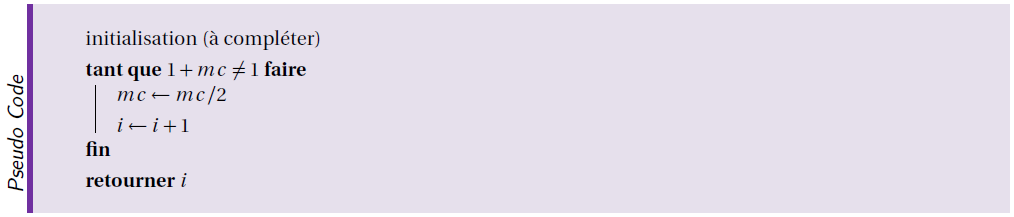
\includegraphics[scale=0.67]{pseudo.png}

\question{
Commenter ou compléter l'algorithme proposé :}
\vspace{-.5cm}
\textit{\begin{itemize}
\item compléter la partie initialisation;
\item justifier le type de boucle choisie;
\item repérer la condition d'arrêt;
\item invariant de boucle;
\item la boucle a-t-elle une fin ?
\item l'algorithme effectue t-il ce que l'on attend ?
\end{itemize}}



\question{Implémenter cet algorithme dans \texttt{python}. Conclure quant au nombre de bits disponibles pour coder la mantisse d'un flottant.}

Il est possible d'appliquer la méthode \texttt{hex()} sur un flottant pour avoir sa représentation en hexadécimal.

\begin{lstlisting}
>>> f = 5.25
>>> f.hex()
        '0x1.5000000000000p+2'
\end{lstlisting}

Cela dit que 5,25 est représentée par le nombre $1\times (5000000000000)_{16} \times 2^{2}$
dont la mantisse est 1,5000000000000 et l'exposant 2.
%\invite rad = 2.0 ** .5\\
%\invite rad.hex ()\\
%'0x1.6a09e667f3bcdp+0'
%La mantisse est 1.6a09e667f3bcdp et l'exposant 0

\question{Déterminer la mantisse de $\sqrt{2}$ à partir de son expression hexadécimale.}

\exer{Génération de nombres pseudo aléatoires}

On se propose d'étudier un algorithme permettant de générer des nombres pseudo-aléatoires.

\subsubsection*{Générer des nombres aléatoires}
Un générateur de nombres aléatoires, \texttt{Random Number Generator} (RNG) en anglais, est un dispositif capable de produire une séquence de nombres dont on ne peut pas « facilement » tirer des propriétés déterministes. Cette fonctionnalité est présente dans Python avec la bibliothèque \texttt{random}.

Des méthodes pour obtenir des nombres aléatoires existent depuis très longtemps et sont utilisées dans les jeux de hasard : dés, roulette, tirage au sort, mélange des cartes, etc... 

\vspace{0.2cm}
Ces générateurs ont une utilité dans de nombreux domaines. Outre les jeux, on peut citer :
\begin{itemize} 
\item la simulation (phénomènes physiques aléatoires);
\item l'échantillonnage;
\item la prise de décision;
\item la sécurité informatique (cryptologie, génération de clé).
\end{itemize}

\vspace{0.5cm}

Les critères suivants permettent de définir la qualité d'un générateur pseudo aléatoire:
\begin{itemize}
%[label=\textbullet]
\item    \textbf{la vitesse} : il faut que le calcul du nombre pseudo-aléatoire suivant soit rapide. Il n'est pas rare de devoir générer des millions de nombres.
\item  \textbf{la méthode ne doit pas souffrir de faille grave} : l'histoire des générateurs pseudo-aléatoire est pleine d'algorithmes qui se « coincent » lorsqu'ils arrivent sur un nombre particulier. Cette situation est source de bogues informatiques qui semblent eux aléatoires et qui sont par conséquent très difficiles à mettre en évidence.

\item   \textbf{les nombres produits ne doivent pas faire apparaître de suite logique}, quelle que soit la façon de les regarder. Ce critère est le plus difficile à quantifier car il dépend fortement de l'application.

\item \textbf{chaque nombre doit apparaitre de manière équiprobable} : c'est-à-dire qu'on doit avoir un nombre de chance équivalent d'obtenir chaque nombre.
\end{itemize}

%\ifProf \begin{commentaire}
%Des infos supplémentaires sur ce site, d'où est issu une partie du texte.
%http://www.alrj.org/docs/algo/random.php
%\end{commentaire} \fi



On dit qu'un générateur pseudo-aléatoire est acceptable s'il a passé avec succès toute une série de tests de statistiques généraux.\\

Nous allons travailler avec l'algorithme de génération de nombres pseudo aléatoires défini par D.H.Lehmer en 1948 : 
\begin{center}
$U_{n+1}=(a \times U_n+c)\text{ mod }(m)$.
\end{center}
Le premier terme $U_0$ est appelé << graine >> (seed en anglais). Les choix du multiplicateur \texttt{a}, de l'incrément \texttt{c}, du module \texttt{m}, et de $U_0$ conditionnent la pertinence des nombres obtenus.\\

Pour la suite du TP, nous prendrons les valeurs suivantes :

$$\left\{ \begin{array}{l}
   U_0=13  \\
   U_{n+1}=f( U_{n})\\
\mbox{où f est une fonction qui a } x \mbox{ associe }
(16805 \times x+1)\texttt{ mod }2^{15}  \\
\end{array} \right.$$

\begin{center}
a mod b désigne le reste dans la division euclidienne de a par b.
\end{center}



\question{\'Ecrire une fonction \texttt{f(u:int)->int} qui à partir du terme $U_n$, renvoie le terme suivant $U_{n+1}$ de la suite. Cette fonction prendra pour argument \texttt{u}. Afficher les 1000 premiers termes de la suite. Les nombres générés vous paraissent-ils aléatoires ?}




\subsubsection*{Génération de booléens}
Nous allons nous servir des nombres pseudo-aléatoires générés pour générer des booléens, par exemple pour simuler une suite de tirages à \texttt{pile} ou \texttt{face}.\\
Nous avons deux situations possibles : soit \texttt{pile}, soit \texttt{face} que l'on peut rapprocher du "0" et du "1" de la représentation binaire.

La méthode consiste à convertir les termes de la suite décrite précédemment en nombres binaires. On extrait alors le n\up{ième} bit du nombre généré (on compte le n\up{ième} bit à partir de la droite).

Si ce bit est à "1" alors le tirage est \texttt{pile}, \texttt{face} dans l'autre cas.

\question{\'Ecrire la fonction \texttt{binaire(e:int)} qui convertit un entier en base 2. 
Cette fonction aura pour argument l'entier \texttt{e} à convertir et retournera une chaine de caractère constituée de 0 et de ~1.\\
Vérifier votre travail en comparant avec la fonction \texttt{bin} de \texttt{python} sur plusieurs exemples.}

\question{\'Ecrire une fonction \texttt{booleen(e:int,n:int)->str} qui convertit un entier \texttt{e} en base 2 et renvoie le n\up{ième} bit sous la forme '0' ou '1' (n\up{ième} bit compté à partir de la droite). \texttt{n} est la position du bit à extraire. Attention, il faut traiter les cas où le nombre obtenu est codé sur moins de \texttt{n} bits !}

%\ifProf \begin{commentaire}
%possibilité d'un if
%\end{commentaire} \fi

\question{On choisit d'utiliser le bit de poids faible (bit des unités) de chaque élément de la suite $U_n$.
Vérifier l'équiprobabilité de la méthode en comptant le nombre de fois que sort le booléen 1 (tirage \texttt{face}) sur un test sur 10000 tirages.
Afficher la liste des 100 premiers termes.\\
Conclure quant à la pertinence du choix du bit de poids le plus faible.}

%\ifProf \begin{commentaire}
%boucles FOR + compteur
%\end{commentaire} \fi

\question{Répondre à la question précédente en choisissant le 9\up{ième} bit.}



\subsubsection*{Génération d'un entier quelconque}
\question{Loin d'être réellement aléatoire, la suite de Lehmer est en fait périodique. On propose d'observer cette propriété. Déterminer au bout de combien de tirages le nombre initial 13 réapparait.
En déduire la période (apparente) de la suite.}


\question{Vérifier que chacun des nombres de l'intervalle des entiers $\llbracket 0,32768 \llbracket$  n'apparaissent qu'une seule fois sur une période. Pour cela, réaliser un programme qui affiche le nombre d'apparitions s'il est différent de 1, et qui affiche \textbf{Tous les nombres apparaissent une seule fois} si c'est le cas.\\ Conclure quant à l'équiprobabilité.}

Remarque : Pour créer une liste ne contenant que des zéros, on peut utiliser la syntaxe suivante:

\begin{lstlisting}
>>> liste = [0]*7  # creation d'une liste avec 7 elements qui valent tous 0
>>> liste
            [0,0,0,0,0,0,0]
\end{lstlisting}




%\ifProf \begin{commentaire}
%si boucles for imbriquées (programmation basique, déconseillée) faire évoluer vers l'emploi d'une liste pour stocker les compteurs
%\end{commentaire} \fi


\question{ (\textit{optionnelle}) Tester la fonction \texttt{randint} de \texttt{python}. Cette fonction est disponible en important la bibliothèque \texttt{random}.  Vous pouvez notamment évaluer sur un échantillon suffisamment grand (100000 tirages par exemple) le nombre d'apparition de quelques entiers.}

%\ifProf \begin{commentaire}
%vraiment pour ceux qui s'ennuient
%
%Pour tester l'homogénéité de la répartition on utilise la quantité ki² suivante: 
%
%$\displaystyle{\sum_{i=1}^r\frac{(f_i-N/r)^2}{N/r}}$
%
%$f_i$ est le nombre d'occurrence de l'entier i
%N est le nombre de tirage
%
%Grossièrement, si la répartition est homogène (cas idéal), chaque entier de [1,r] est généré N/r fois, et cette quantité est donc nulle.
%\end{commentaire} \fi


Le 9\up{ième} bit permet de générer une séquence suffisamment aléatoire de \texttt{pile} et de \texttt{face} suivant les critères donnés en introduction. Malheureusement, puisque l'on part toujours de $U_0=13$, la séquence générée est toujours la même. On souhaite donc créer un entier $U_0$ compris entre 0 et $2^{15}-1$, qui serait aléatoire.

\question{Proposer une méthode pour créer un tel entier, en se servant de la fonction \texttt{time.perf\_counter()} ou \texttt{time.perf\_counter\_ns()} (voir en bas de page).\\
\'Ecrire une fonction \texttt{graine()} qui retourne cet entier aléatoire.\\
\'Ecrire une fonction \texttt{aleatoire(n:int)} qui génère une liste de n \texttt{pile} et \texttt{face} (0 et 1) obtenue avec le 9\up{ième} bit, en partant de cet entier aléatoire. Cette fonction prendra comme argument le nombre \texttt{n} de booléens voulus (taille de la liste à retourner).
}


\vspace{0.5cm}
\texttt{time.perf\_counter() → float}\\
Return the value (in fractional seconds) of a performance counter, i.e. a clock with the highest available resolution to measure a short duration.

\texttt{time.perf\_counter\_ns() → int:}\\
Similar to perf\_counter(), but return time as nanoseconds (new in version 3.7).

\texttt{time.process\_time() → float}\\
Return the value (in fractional seconds) of the sum of the system and user CPU time of the current process.

\texttt{time.process\_time\_ns() → int}\\
Similar to process\_time() but return time as nanoseconds.






\end{document}



